\documentclass[twoside,11pt]{homework}

\coursename{EECS E6892 Fall 2015} % DON'T CHANGE THIS

\studentname{Daniel Kronovet}       % YOUR NAME GOES HERE
\studentmail{dbk2123@columbia.edu}   % YOUR UNI GOES HERE
\homeworknumber{1}               % THE HOMEWORK NUMBER GOES HERE
\collaborators{Stephen Ra, Sam Guleff, Steve Royce, Elliot Oh}             % THE UNI'S OF STUDENTS YOU DISCUSSED WITH

\begin{document}
\maketitle

\section*{Problem 1}

We will approach the problem by first choosing a door, and then calculating the probability that the door contains the prize after observing another door.

First, our variables. Let $\theta = i$ denote the odds that the prize is behind door $i$, $X=j$ denote the even that we observe the contents of door $j$, and $P(X=j | \theta=i)$ denote the likelihood that we would have observed the contents of door $j$ given the existence a prize behind door $i$.

Let us begin by guessing that the prize is behind door 1, something which a priori has an odds of 1/3. Then we see the contents of door 2, which is empty. Knowing this, we can determine the odds that the prize is behind door 1. Implicit is the fact that the likelihood of observing the contents of the door we have picked, or the door actually containing the prize, is 0. We can calculate the odds as follows:

\[
\frac{P(X=2 | \theta=1)P(\theta = 1)}{P(X=2 | \theta=1)P(\theta = 1) + P(X=2 | \theta=2)P(\theta = 2) + P(X=2 | \theta=3)P(\theta = 3)} = P(\theta = 1 | X=2)
\]


\[
\frac{(1/2)(1/3)}{(1/2)(1/3) + (0)(1/3) + (1)(1/3)} = \frac{1/6}{1/6 + 1/3} = 1/3
\]

\section*{Problem 2}

We begin with $X \sim Multinomial(\pi)$. This distribution, a generalization of the binomial distribution from 2 to $k$ categories, represents the likelihood of a specific combination of $n$ discrete events across $k$ different categories. The multinomial is parameterized by model variable $\pi$, a $k$-dimensional vector of probabilities, one for each category, and summing to 1. We can represent $X$ as $\sum^n{X_i}$, with each $X_i$ representing one observance (a vector of size $k$ with a 1 in the location of the category of the observance, and 0 elsewhere), and $\sum_{j=1}^k X_j = n$. The total number of observances for category $j$ will be denoted $x_j$, to distinguish from $X_j$, the $jth$ observation.

We wish to find a conjugate prior distribution on $\pi$, so that after observing some arbitrary number of trials, we can easily update the distribution of $\pi$ to more accurately reflect the realty we have observed. The Dirichlet distribution will serve as a prior. The Dirichlet is (appropriately), the multivariate generalization of the Beta distribution, providing us with a distribution on a $k$-sized vector of probabilities (each between 0 and 1), parameterized by $\alpha$, a $k$-sized vector of event observations. In other words, we can think of the Multinomial distribution as giving the likelihood of a set of observations given specific event probabilities, and the Dirichlet as giving the likelihood of specific event probabilities given a set of observations.

We now derive the posterior:

\[
P(\pi | X, \alpha) = \frac{P(X|\pi)P(\pi|\alpha)}{\int P(X|\pi)P(\pi|\alpha) d\pi}
\]

Considering first the numerator (the product of the likelihood and the prior):

\[
P(X|\pi)P(\pi|\alpha) = \Parens{\frac{n!}{\prod^k x_i!}\prod^k \pi_i^{x_i}}\Parens{\frac{\Gamma(\sum^k \alpha_i)}{\prod^k \Gamma(\alpha_i)}\prod^k \pi_i^{\alpha_i - 1}}
\]

\[
\frac{n!}{\prod^k x_i!}\frac{\Gamma(\sum^k \alpha_i)}{\prod^k \Gamma(\alpha_i)}\prod^k \pi_i^{x_i}\prod^k \pi_i^{\alpha_i - 1}
\]

\[
\frac{n!}{\prod^k x_i!}\frac{\Gamma(\sum^k \alpha_i)}{\prod^k \Gamma(\alpha_i)}\prod^k \pi_i^{x_i + \alpha_i - 1}
\]

Observe that we now have a Dirichlet distribution $\sim Dir(X + \alpha)$, scaled by a constant term.

\[
P(\pi | X, \alpha) = 
\frac{
\frac{n!}{\prod^k x_i!}\frac{\Gamma(\sum^k \alpha_i)}{\prod^k \Gamma(\alpha_i)}\prod^k \pi_i^{x_i + \alpha_i - 1}
}{
\int \frac{n!}{\prod^k x_i!}\frac{\Gamma(\sum^k \alpha_i)}{\prod^k \Gamma(\alpha_i)}\prod^k \pi_i^{x_i + \alpha_i - 1} d\pi
}
\]

Canceling like terms gives:

\[
P(\pi | X, \alpha) = 
\frac{
\prod^k \pi_i^{x_i + \alpha_i - 1}
}{
\int \prod^k \pi_i^{x_i + \alpha_i - 1} d\pi
}
\]

We know that this term must integrate to 1, as it is a probability distribution on $\pi$.
This implies that the denominator, which integrates to a constant, must integrate to the reciprocal of the normalizing constant
for the Dirichlet distribution. Thus, this expression evaluates to:

\[
P(\pi | X, \alpha) = 
\frac{\Gamma(n + \sum^k \alpha_i)}{\prod^k \Gamma(x_i + \alpha_i)}
\prod^k \pi_i^{x_i + \alpha_i - 1}
\]

Which is our desired posterior, conjugate with the prior.

\section*{Problem 3}
\textbf{Part a}

We begin with two distributions, one $\mu \sim N(m, (a\lambda)^{-1})$ and one $\lambda \sim Gamma(b, c)$, which we multiply together to get a prior joint distribution on $\mu, \lambda$:

\[
\frac{1}{\sqrt{2\pi(a\lambda)^{-1}}}
exp[-\frac{1}{2}a\lambda(\mu - m)^2]
\frac{c^b}{\Gamma{(b)}}
\lambda^{b-1}
exp[-c\lambda]
\]

\[
\frac{(a\lambda)^{1/2}}{\sqrt{2\pi}}
\frac{c^b}{\Gamma{(b)}}
\lambda^{b-1}
exp[-c\lambda]
exp[-\frac{1}{2}a\lambda(\mu - m)^2]
\]

\[
\frac{\sqrt{a}}{\sqrt{2\pi}}
\frac{c^b}{\Gamma{(b)}}
\lambda^{b-1+\frac{1}{2}}
exp[-c\lambda]
exp[-\frac{1}{2}a\lambda(\mu - m)^2]
\]

Thus we are able to derive the Normal-gamma distribution:

\[
\frac{c^b\sqrt{a}}{\Gamma{(b)}\sqrt{2\pi}}
\lambda^{b-\frac{1}{2}}
exp[-c\lambda]
exp[-\frac{1}{2}a\lambda(\mu - m)^2]
\]

Moving on, we now want to derive the posterior Normal-gamma.
We begin by multiplying the Normal-gamma prior with our data, modeled $x_i \sim N(\mu, \lambda^{-1})$

\[
\Parens{
\prod^n
\frac{\sqrt{\lambda}}{\sqrt{2\pi}}
exp[-\frac{1}{2}\lambda(x_i - \mu)^2]
}
\Parens{
\frac{c^b\sqrt{a}}{\Gamma{(b)}\sqrt{2\pi}}
\lambda^{b-\frac{1}{2}}
exp[-c\lambda]
exp[-\frac{1}{2}a\lambda(\mu - m)^2]
}
\]

\[
\Parens{
\frac{\lambda^{n/2}}{(2\pi)^{n/2}}
exp[-\frac{1}{2}\lambda\sum^n(x_i - \mu)^2]
}
\Parens{
\frac{c^b\sqrt{a}}{\Gamma{(b)}\sqrt{2\pi}}
\lambda^{b-\frac{1}{2}}
exp[-c\lambda]
exp[-\frac{1}{2}a\lambda(\mu - m)^2]
}
\]

Combining terms:

\[
\frac{c^b\sqrt{a}}{\Gamma{(b)}(2\pi)^{\frac{n+1}{2}}}
\lambda^{(b+\frac{n}{2})-\frac{1}{2}}
exp[-c\lambda]
exp[-\frac{1}{2}\lambda
\Parens{a(\mu - m)^2 + \sum^n(x_i - \mu)^2}
]
\]

Considering the the exponent, we complete the square to get a distribution over $\mu$.

\[
a(\mu - m)^2 + \sum^n(x_i - \mu)^2
\]

First, note that the summation can be simplified in the following way:

\[
\sum^n(x_i - \mu)^2 = \sum^n(x_i + \bar{x} - \bar{x} - \mu)^2 = \sum^n (x_i - \bar{x})^2 + \sum^n (\bar{x} - \mu)^2
\]

This manipulation relies on the equality between $\sum x \bar{x} = \sum \bar{x} \bar{x}$ and $\sum x \mu = \sum \bar{x} \mu$.
Summing the terms, we get:

\[
ns + n(\bar{x} - \mu)^2
\]

With $s = \frac{1}{n} \sum^n (x_i - \bar{x})^2$, the sample variance.

With this, we return to the previous term:

\[
a(\mu - m)^2 + ns + n(\bar{x} - \mu)^2
\]

Expanding and organizing, we see:

\[
a\mu^2 - a2\mu m + am^2 + ns + n\bar{x}^2 - n2\bar{x}\mu + n\mu^2
\]

\[
(a+n)\Parens{\mu^2 - 2\mu \frac{(am + n\bar{x})} {(a+n)}}
+ am^2 + ns + n\bar{x}^2
\]

Completing the square:

\[
(a+n)
\Parens{
\mu^2 - 2\mu \frac{(am + n\bar{x})}{(a+n)} + \Parens{\frac{(am + n\bar{x})}{(a+n)}}^2
} - \frac{(am + n\bar{x})^2}{(a+n)} + am^2 + ns + n\bar{x}^2
\]

\[
(a+n)
\Parens{
\mu - \frac{(am + n\bar{x})}{(a+n)}
}^2 - \frac{(am + n\bar{x})^2}{(a+n)} + am^2 + ns + n\bar{x}^2
\]

Which simplifies to:

\[
(a+n)
\Parens{
\mu - \frac{(am + n\bar{x})}{(a+n)}
}^2 + \frac{na(\bar{x} - m)^2}{(a+n)} + ns
\]

Returning to the full numerator, we have:

\[
\frac{c^b\sqrt{a}}{\Gamma{(b)}(2\pi)^{\frac{n+1}{2}}}
\lambda^{(b+\frac{n}{2})-\frac{1}{2}}
exp[-c\lambda]
exp[-\frac{1}{2}\lambda
\Parens{
(a+n)
\Parens{
\mu - \frac{(am + n\bar{x})}{(a+n)}
}^2 + \frac{na(\bar{x} - m)^2}{(a+n)} + ns
}]
\]

\[
\frac{c^b\sqrt{a}}{\Gamma{(b)}(2\pi)^{\frac{n+1}{2}}}
\lambda^{(b+\frac{n}{2})-\frac{1}{2}}
exp[-\lambda \Parens{c + \frac{na(\bar{x} - m)^2}{2(a+n)} + ns/2}]
exp[-\frac{1}{2}\lambda
\Parens{
(a+n)
\Parens{
\mu - \frac{(am + n\bar{x})}{(a+n)}
}^2}]
\]

This posterior is conjugate to the Normal-Gamma prior on $\mu, \lambda$, allowing us to perform updates by calculating the following sufficient statistics:

\[
a^* = a+n
\]
\[
b^* = b + n/2
\]
\[
c^* = c + \frac{1}{2}\Parens{\frac{na(\bar{x} - m)^2}{(a+n)} + ns}
\]
\[
m^* = \frac{(am + n\bar{x})}{(a+n)}
\]

Describing the posterior using the updated terms, we are left with:

\[
p(\mu, \lambda | a, b, c, m, \bfX) = 
\frac{
\frac{c^b\sqrt{a}}{\Gamma{(b)}(2\pi)^{\frac{n+1}{2}}}
\lambda^{(b^*)-\frac{1}{2}}
exp[-\lambda c^*]
exp[-\frac{1}{2}\lambda a^*
\Parens{
\mu - m^*
}^2]
}
{\int \int
\frac{c^b\sqrt{a}}{\Gamma{(b)}(2\pi)^{\frac{n+1}{2}}}
\lambda^{(b^*)-\frac{1}{2}}
exp[-\lambda c^*]
exp[-\frac{1}{2}\lambda a^*
\Parens{
\mu - m^*
}^2]
d\mu d\lambda
}
\]

Canceling out the constants which do not depend on $\mu, \lambda$:

\[
\frac{
\lambda^{(b^*)-\frac{1}{2}}
exp[-\lambda c^*]
exp[-\frac{1}{2}\lambda a^*
\Parens{
\mu - m^*
}^2]
}
{\int \int
\lambda^{(b^*)-\frac{1}{2}}
exp[-\lambda c^*]
exp[-\frac{1}{2}\lambda a^*
\Parens{
\mu - m^*
}^2]
d\mu d\lambda
}
\]

Given that this term evaluates to $p(\mu, \lambda | a, b, c, m, \bfX)$, which integrates to 1,
we know that this expression must also integrate to 1.
This implies denominator must integrate to a constant:
specifically, to the reciprocal of the normalizing constant 
for the updated Normal-Gamma distribution, ultimately giving:

\[
\frac{c^{* b^*}\sqrt{a^*}}{\Gamma{(b^*)}\sqrt{2\pi}}
\lambda^{(b^*)-\frac{1}{2}}
exp[-\lambda c^*]
exp[-\frac{1}{2}\lambda a^*
\Parens{
\mu - m^*
}^2]
\]

\textbf{Part b}

In this problem, we will derive the predictive distribution on new observation $x^*$, with:

\[
p(x^*|\bfX) = \int_{0}^{\infty}\int_{-\infty}^{\infty} p(x^*|\mu, \lambda)p(\mu, \lambda | a, b, c, m, \bfX) d\mu d\lambda
\]

Given that $\mu, \lambda \sim Normal-Gamma(a, b, c)$, we can decompose the integral into the following:
\[
p(x^*|\bfX) = \int_{0}^{\infty}\int_{-\infty}^{\infty} p(x^*|\mu, \lambda)p(\mu | m, a, \lambda, \bfX) p(\lambda | b, c, \bfX)d\mu d\lambda
\]

With $x^* \sim N(\mu, \lambda^{-1}), \mu \sim N(m, (a\lambda)^{-1}), \lambda \sim Gamma(b, c)$.
In implementation, $a, b, c, m$ will incorporate the information from $\bfX$,
so for simplicity we will exclude $\bfX$ from this derivation, leaving:
\[
p(x^*|a, b, c, m) = \int_{0}^{\infty}\int_{-\infty}^{\infty} p(x^*|\mu, \lambda)p(\mu | m, a, \lambda) p(\lambda | b, c )d\mu d\lambda
\]


Our approach to this problem will be to first integrate out $\mu$, and then $\lambda$.
To do this, we will first combine the two normal distributions into a single normal distribution, which we will integrate to 1. Rearranging:

\[
p(x^*|a, b, c, m) =
\int_{0}^{\infty} p(\lambda | b, c )\Parens{\int_{-\infty}^{\infty} p(x^*|\mu, \lambda)p(\mu | m, a, \lambda) d\mu} d\lambda
\]

First we consider the inner integral:

\[
\int_{-\infty}^{\infty} p(x^*|\mu, \lambda)p(\mu | m, a, \lambda) d\mu
\]


\[
\int_{-\infty}^{\infty}
\frac{\sqrt{\lambda}}{\sqrt{2\pi}}
exp\braces{-\frac{1}{2}\lambda(x^* - \mu)^2}
\frac{\sqrt{a\lambda}}{\sqrt{2\pi}}
exp\braces{-\frac{1}{2}a\lambda(\mu - m)^2}
d\mu
\]

\[
\int_{-\infty}^{\infty}
\frac{\sqrt{\lambda}}{\sqrt{2\pi}}
\frac{\sqrt{a\lambda}}{\sqrt{2\pi}}
exp\braces{-\frac{1}{2}\lambda(x^* - \mu)^2 -\frac{1}{2}a\lambda(\mu - m)^2}
d\mu
\]

\[
\int_{-\infty}^{\infty}
\frac{\sqrt{\lambda}}{\sqrt{2\pi}}
\frac{\sqrt{a\lambda}}{\sqrt{2\pi}}
exp\braces{-\frac{1}{2}\lambda[(x^* - \mu)^2 + a(\mu - m)^2]}
d\mu
\]

Now considering only the terms in the square brackets,
we would like to get an expression of the form $(\mu - y)^2 + z$:

\[
(x^* - \mu)^2 + a(\mu - m)^2
\]

\[
x^{*2} - 2x^*\mu + \mu^2 + a(\mu^2 - 2\mu m + m^2)
\]


\[
x^{*2} - 2x^*\mu + \mu^2 + a\mu^2 - a2\mu m + am^2
\]

Regrouping, we have:

\[
a\mu^2 + \mu^2 - 2x^*\mu - a2\mu m + x^{*2} + am^2
\]

\[
(a + 1)\mu^2 - 2\mu(x^* + am) + x^{*2} + am^2
\]

From here we can complete the square:

\[
(a + 1)\Parens{\mu^2 - 2\mu\frac{(x^* + am)}{a+1}} + x^{*2} + am^2
\]

\[
(a + 1)
\Parens{\mu^2 - 2\mu\frac{(x^* + am)}{a+1} + \frac{(x^* + am)^2}{(a+1)^2} - \frac{(x^* + am)^2}{(a+1)^2}}
 + x^{*2} + am^2
\]

\[
(a + 1)
\Parens{\mu^2 - 2\mu\frac{(x^* + am)}{a+1} + \frac{(x^* + am)^2}{(a+1)^2}}
- \frac{(x^* + am)^2}{(a+1)} + x^{*2} + am^2
\]

\[
(a + 1)
\Parens{\mu - \frac{(x^* + am)}{a+1}}^2
- \frac{(x^* + am)^2}{(a+1)} + x^{*2} + am^2
\]

And then simplify the remaining terms:

\[
(a + 1)
\Parens{\mu - \frac{(x^* + am)}{a+1}}^2
- \frac{x^{*2} + 2x^*am + a^2m^2}{(a+1)^2} + \frac{ax^{*2} + a^2m^2 + x^{*2} + am^2}{(a + 1)^2}
\]

\[
(a + 1)
\Parens{\mu - \frac{(x^* + am)}{a+1}}
+ \frac{- x^{*2} - 2x^*am - a^2m^2 + ax^{*2} + a^2m^2 + x^{*2} + am^2}{(a + 1)}
\]

\[
(a + 1)
\Parens{\mu - \frac{(x^* + am)}{a+1}}
+ \frac{- 2x^*am + ax^{*2} + am^2}{(a + 1)}
\]

\[
(a + 1)
\Parens{\mu - \frac{(x^* + am)}{a+1}}
+ \frac{a(-2x^*m + x^{*2} + m^2)}{(a + 1)}
\]

\[
(a + 1)
\Parens{\mu - \frac{(x^* + am)}{a+1}}
+ \frac{a(x^* - m)^2}{(a + 1)}
\]

Now, returning to the original expression:

\[
\int_{-\infty}^{\infty}
\frac{\sqrt{\lambda}}{\sqrt{2\pi}}
\frac{\sqrt{a\lambda}}{\sqrt{2\pi}}
exp\Braces{-\frac{1}{2}\lambda
\Brackets{
(a + 1)
\Parens{\mu - \frac{(x^* + am)}{a+1}}^2
+ \frac{a(x^* - m)^2}{(a + 1)}}
}
d\mu
\]

\[
\int_{-\infty}^{\infty}
\frac{\sqrt{\lambda}}{\sqrt{2\pi}}
\frac{\sqrt{a\lambda}}{\sqrt{2\pi}}
exp\Braces{
-\frac{1}{2}\lambda
(a + 1)
\Parens{\mu - \frac{(x^* + am)}{a+1}}^2
- \frac{1}{2}\lambda
\Parens{\frac{a(x^* - m)^2}{(a + 1)}}
}
d\mu
\]

\[
\int_{-\infty}^{\infty}
\frac{\sqrt{\lambda}}{\sqrt{2\pi}}
\frac{\sqrt{a\lambda}}{\sqrt{2\pi}}
exp\Braces{
-\frac{1}{2}\lambda
(a + 1)
\Parens{\mu - \frac{(x^* + am)}{a+1}}^2
}
exp\Braces{
- \frac{1}{2}\lambda
\Parens{\frac{a(x^* - m)^2}{(a + 1)}}
}
d\mu
\]

\[
\frac{\sqrt{a\lambda}}{\sqrt{2\pi(a+1)}}
exp\Braces{
- \frac{1}{2}\lambda
\Parens{\frac{a(x^* - m)^2}{(a + 1)}}
}
\int_{-\infty}^{\infty}
\frac{\sqrt{\lambda(a+1)}}{\sqrt{2\pi}}
exp\Braces{
-\frac{1}{2}\lambda
(a + 1)
\Parens{\mu - \frac{(x^* + am)}{a+1}}^2
}
d\mu
\]

The integrand is now a normal distribution, and thus integrates to 1:

\[
\frac{\sqrt{a\lambda}}{\sqrt{2\pi(a+1)}}
exp\Braces{
- \frac{1}{2}\lambda
\Parens{
\frac{a(x^* - m)^2}{(a + 1)}
}
}
\]

We now return to the full expression:

\[
p(x^*|a, b, c, m) =
\int_{0}^{\infty}
p(\lambda | b, c )
\frac{\sqrt{a\lambda}}{\sqrt{2\pi(a+1)}}
exp\Braces{
- \frac{1}{2}\lambda
\Parens{
\frac{a(x^* - m)^2}{(a + 1)}
}
}d\lambda
\]

We introduce the Gamma distribution:

\[
\int_{0}^{\infty}
\frac{c^b}{\Gamma(b)}
\lambda^{b-1}
exp\Braces{
-c\lambda
}
\frac{\sqrt{a\lambda}}{\sqrt{2\pi(a+1)}}
exp\Braces{
- \frac{1}{2}\lambda
\Parens{
\frac{a(x^* - m)^2}{(a + 1)}
}
}d\lambda
\]

Reorganizing terms, we have:

\[
\int_{0}^{\infty}
\frac{c^b}{\Gamma(b)}
\frac{\sqrt{a}}{\sqrt{2\pi(a+1)}}
\lambda^{1/2}
\lambda^{b-1}
exp\Braces{
-c\lambda
- \frac{1}{2}\lambda
\Parens{
\frac{a(x^* - m)^2}{(a + 1)}
}
}d\lambda
\]

\[
\int_{0}^{\infty}
\frac{c^b}{\Gamma(b)}
\frac{\sqrt{a}}{\sqrt{2\pi(a+1)}}
\lambda^{(b+1/2)-1}
exp\Braces{
-\lambda
\Parens{
c
+ \frac{1}{2}
\Parens{
\frac{a(x^* - m)^2}{(a + 1)}
}
}
}d\lambda
\]

Here we have a Gamma distribution with updated parameters:

\[
b^\prime = b + 1/2
\]

\[
c^\prime =  \Parens{
c + \frac{a}{2}
\Parens{
\frac{(x^* - m)^2}{a + 1}
}
}
\]

In order to integrate this distribution to 1, we need to introduce the correct normalizing constant:

\[
\int_{0}^{\infty}
\frac{c^b}{\Gamma(b)}
\frac{\sqrt{a}}{\sqrt{2\pi(a+1)}}
\lambda^{b^\prime-1}
exp\Braces{
-\lambda c^\prime
}d\lambda
\]

\[
\frac{c^b}{\Gamma(b)}
\frac{\sqrt{a}}{\sqrt{2\pi(a+1)}}
\int_{0}^{\infty}
\frac{c^{\prime b^\prime}}{\Gamma(b^\prime)}
\frac{\Gamma(b^\prime)}{c^{\prime b^\prime}}
\lambda^{b^\prime-1}
exp\Braces{
-\lambda c^\prime
}d\lambda
\]

\[
\frac{\Gamma(b^\prime)}{c^{\prime b^\prime}}
\frac{c^b}{\Gamma(b)}
\frac{\sqrt{a}}{\sqrt{2\pi(a+1)}}
\int_{0}^{\infty}
\frac{c^{\prime b^\prime}}{\Gamma(b^\prime)}
\lambda^{b^\prime-1}
exp\Braces{
-\lambda c^\prime
}d\lambda
\]

The integrand now evaluates to 1, leaving us with:

\[
\frac{\Gamma(b^\prime)}{c^{\prime b^\prime}}
\frac{c^b}{\Gamma(b)}
\frac{\sqrt{a}}{\sqrt{2\pi(a+1)}}
\]

\[
\frac{\Gamma(b + 1/2)}{\Gamma(b)}
\frac{\sqrt{a}}{\sqrt{2\pi(a+1)}}
\frac{c^b}{
\Parens{c + \frac{a}{2}
\frac{(x^* - m)^2}{a + 1}}^{b + 1/2}}
\]

Which is a Student's-t distribution, our desired result.

\section*{Problem 4}

\textbf{Part a}

I did this it was fun.

\textbf{Part b}

\begin{center}
  \begin{tabular}{c||c|c|c|c}
    & 0
    & 1 \\
    \hline
    \hline
    $0$
    & 930
    & 52
    \\
    \hline
    $1$
    & 82
    & 927
  \end{tabular}
\end{center}

\[
Accuracy = 0.932697137117
\]

\textbf{Part c}

Image 40:

Prediction: 1

Confidence: 6.2632846920514565e+24

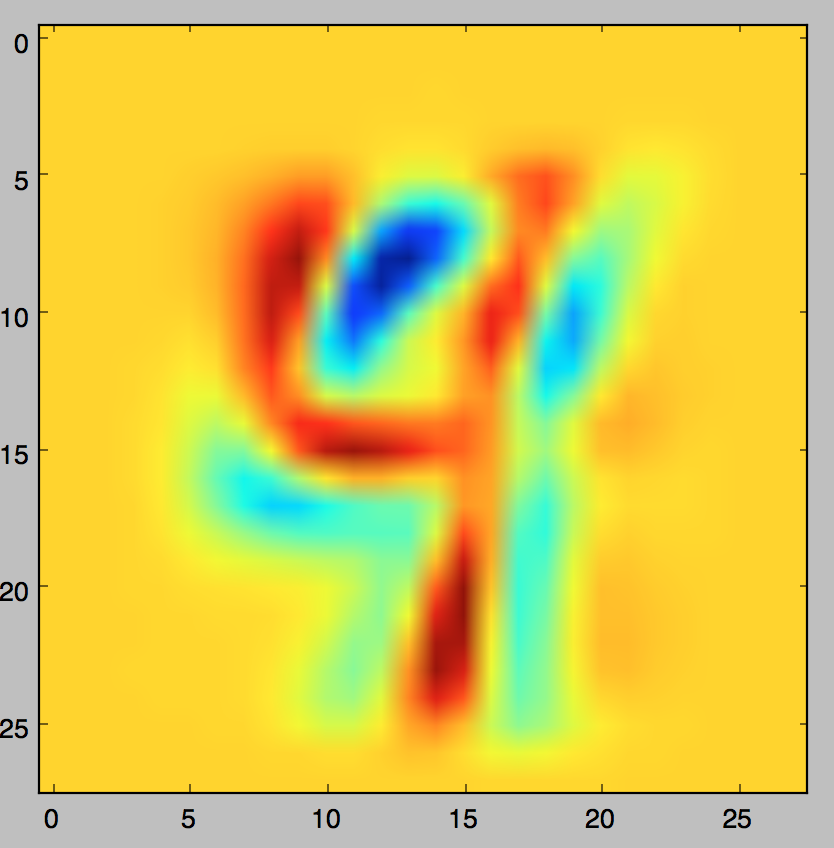
\includegraphics[scale=.5]{images/40.png}

Image 1647:

Prediction: 0

Confidence: 1.9399197255647452e+21

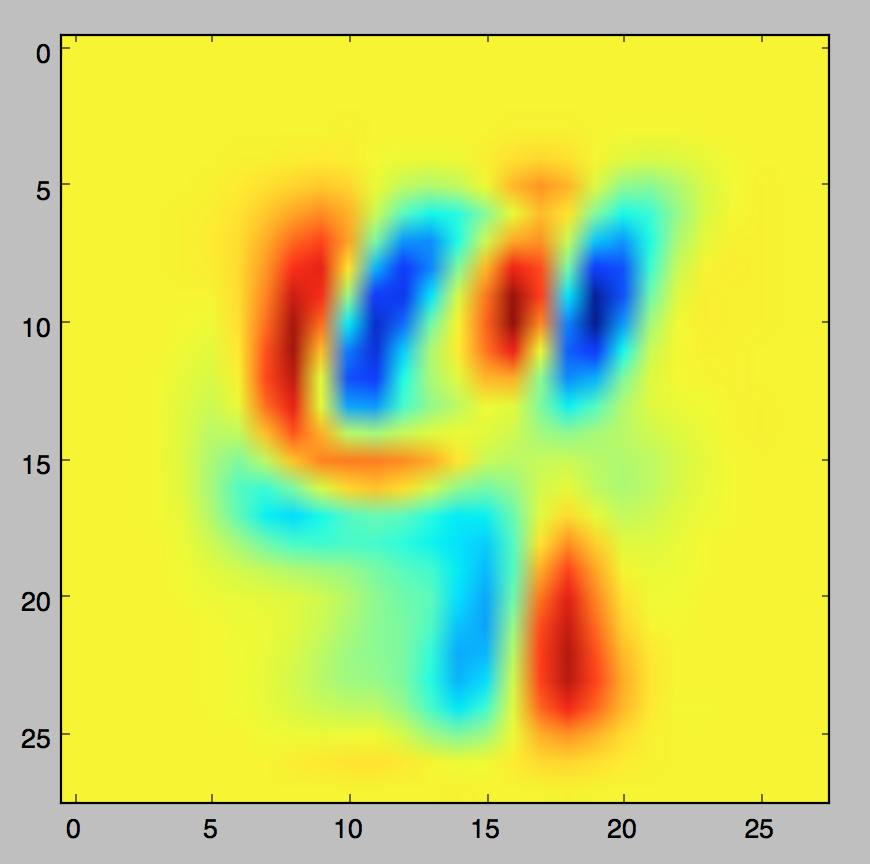
\includegraphics[scale=.5]{images/1647.png}

Image 696:

Prediction: 1

Confidence: 1.7836568232571003e+26

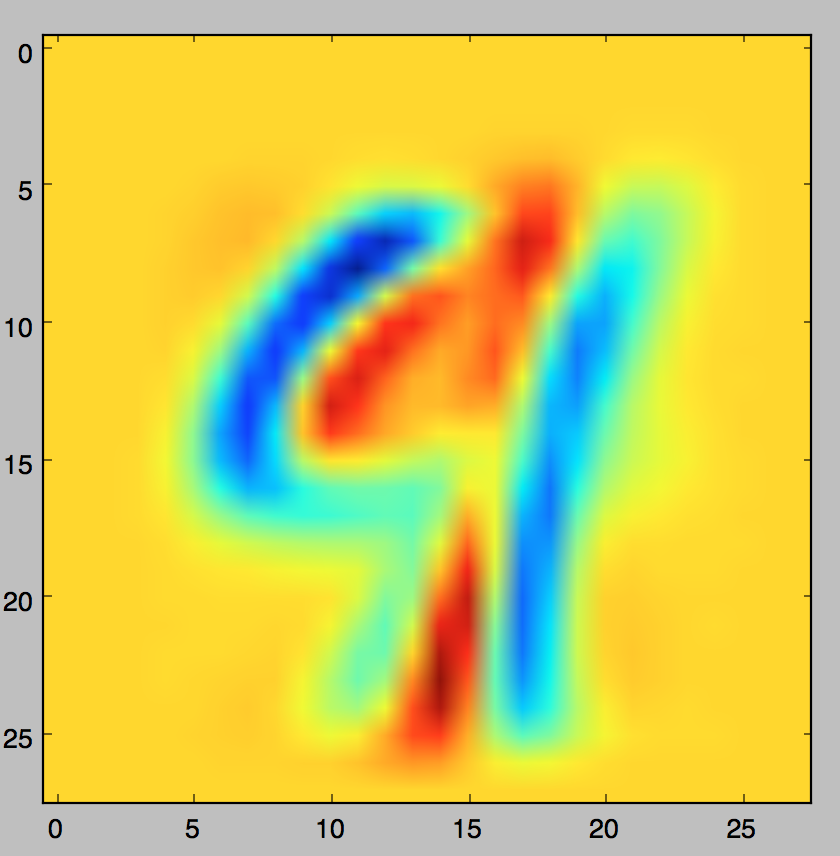
\includegraphics[scale=.5]{images/696.png}

\textbf{Part d}

For this problem I normalized the prediction confidences in the following way.
First I centered the predictions by subtracting off the mean.
Then, I divided by the maximum confidence to bring all confidences $\in (0, 1]$.
Then I took the absolute value of the centered predictions, and then I sorted the predictions.

This gave a list of predictions $\in (0, 1]$. Taking the three  smallest values gave the three most ambiguous predictions.

Most ambiguous:

Image 1883, confidence 0.000035

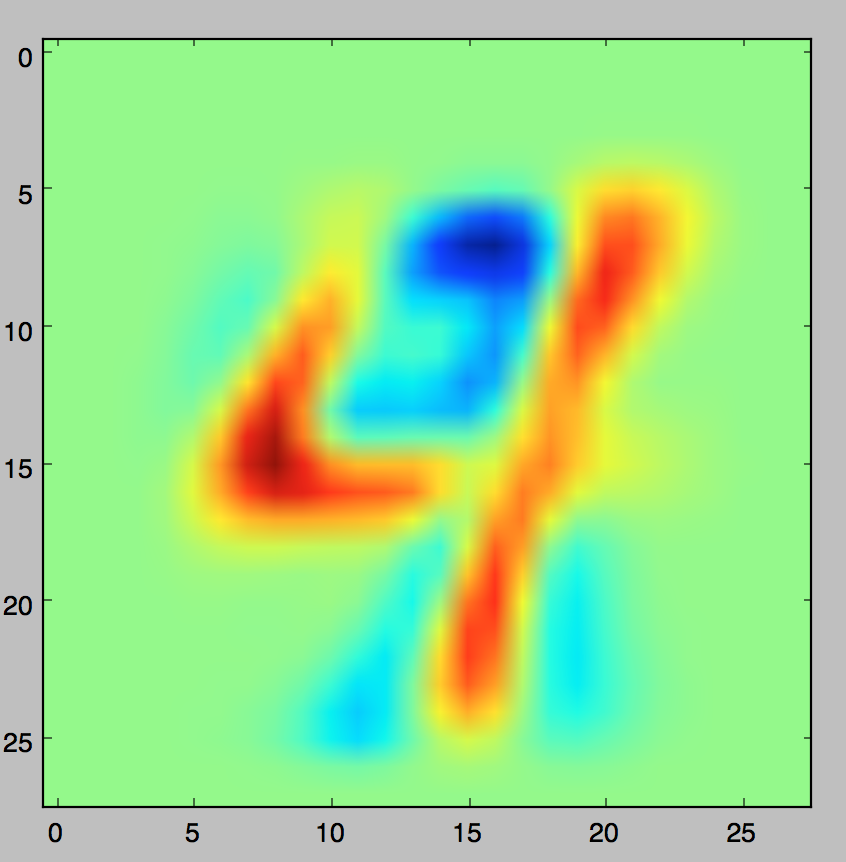
\includegraphics[scale=.5]{images/1883.png}

Image 1555, confidence 0.000171

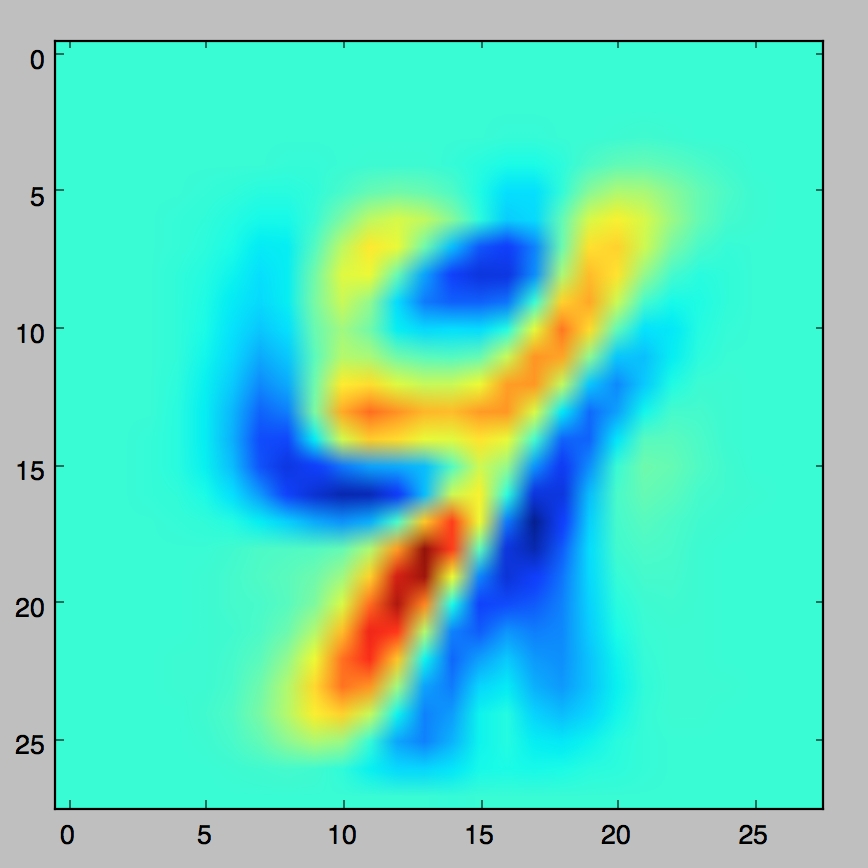
\includegraphics[scale=.5]{images/1555.png}

Image 1766, confidence 0.000337

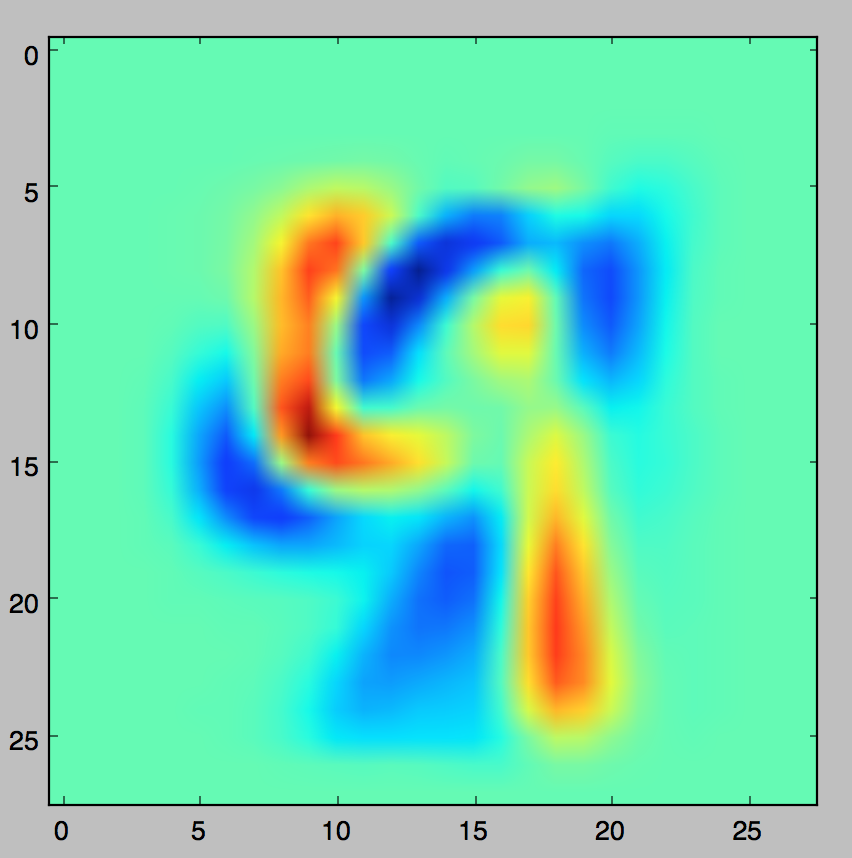
\includegraphics[scale=.5]{images/1766.png}

\end{document} 
